\documentclass[10pt,a4paper,twocolumn]{article}

\usepackage[a4paper,margin=1.4cm,columnsep=0.5cm]{geometry}
\usepackage[T1]{fontenc}
\usepackage{lmodern}
\usepackage{microtype}
\usepackage{graphicx}
\usepackage{booktabs}
\usepackage{amsmath}
\usepackage{amssymb}
\usepackage{xcolor}
\usepackage{caption}
\usepackage{hyperref}
\usepackage{titlesec}

\hypersetup{colorlinks=true,linkcolor=blue!50!black,citecolor=blue!50!black,urlcolor=blue!50!black}

\titlespacing*{\section}{0pt}{0.9ex}{0.3ex}
\titlespacing*{\subsection}{0pt}{0.6ex}{0.2ex}
\titleformat{\section}{\normalsize\bfseries}{\thesection.}{0.4em}{}
\titleformat{\subsection}{\small\bfseries}{\thesubsection.}{0.4em}{}

\captionsetup{font=footnotesize,labelfont=bf,skip=1pt}
\setlength{\parskip}{1pt}
\setlength{\parindent}{0pt}
\setlength{\textfloatsep}{4pt}
\setlength{\floatsep}{4pt}
\setlength{\intextsep}{4pt}

\title{\vspace{-1.5em}\textbf{Real-Time Lane Detection and Autonomous Steering:\\
A Comparison of Classical Pipelines and a Polynomial-Fit Improvement}}
\author{David Tovmasyan \quad\textbullet\quad \href{mailto:david.tovmasyan@connectto.com}{david.tovmasyan@connectto.com}}
\date{}

\begin{document}
\twocolumn[
  \begin{@twocolumnfalse}
    \maketitle
    \vspace{-2.5em}
  \end{@twocolumnfalse}
]

\begin{abstract}\small
\noindent
We design, implement and evaluate a real-time lane detection and
autonomous steering system in a custom 2D driving simulator. Three
classical lane detectors of increasing sophistication---a colour
centroid, a Hough-line pipeline, and a proposed bird's-eye-view +
sliding-window polynomial fit---are paired with a PID steering
controller; a Stanley controller driven from ground-truth track
geometry is added as a perception-free oracle. Across five tracks the
polynomial-fit detector reduces RMS lateral error by
\textbf{34--40\,\%} relative to the Hough baseline (15.7\,px vs.\
25.4\,px on average) while doubling the mean lane-IoU. It is the only
classical detector that survives every noise level we tested
($\sigma\!\le\!0.20$ of pixel intensity). The full pipeline runs above
500\,FPS on a single CPU thread.
\end{abstract}

\section{Problem and motivation}

Lane keeping is the most heavily-deployed autonomous-driving function.
While learned segmenters (LaneNet, SCNN, PolyLaneNet) dominate
benchmarks, a tuned \emph{classical} pipeline remains attractive: it is
fully interpretable, runs at hundreds of FPS on a CPU, and exposes
every assumption it is making. This project asks a concrete question:
\emph{how much performance is left on the table by the textbook
Canny+Hough lane detector, and can a modest polynomial-fit upgrade
close the gap on curved tracks while staying real-time?}

To answer it we (i)~build a 2D forward-perspective driving simulator
that exposes ground-truth geometry, (ii)~implement three lane detectors
behind a shared interface, (iii)~implement PID and Stanley controllers,
and (iv)~run a headless evaluator that sweeps every
(detector,~controller,~track) combination plus a noise-robustness
experiment, logging lateral error, lane-IoU, detection confidence and
inference time per frame.

\section{Method}

\subsection{Simulator and ground truth}
The track is a closed-loop Catmull--Rom spline through hand-placed
waypoints and is rendered through a calibrated pinhole camera with
$70^{\circ}$ FoV, $18^{\circ}$ pitch and $50$\,px camera height. The
vehicle follows the bicycle kinematic model
$\dot{\theta}=(v/L)\tan\delta$ with $L=25$\,px and
$|\delta|\!\leq\!40^\circ$. Five tracks of increasing curvature are
used: Simple Oval, Stadium Circuit, Winding Road, Grand Prix Circuit,
Highland Rally. Ground-truth lateral offset and the ground-truth lane
polygon (used for IoU) are computed analytically from the spline.

\subsection{Baseline 1 -- Centroid}
Threshold the road colour in HSV $(S\!<\!40,\,40\!<\!V\!<\!110)$, mask
a trapezoidal ROI, and use the centroid of the resulting blob (via
image moments) as the lane centre. The simplest detector we could
write down; a deliberate \emph{lower bound}.

\subsection{Baseline 2 -- Hough lines}
The textbook pipeline from the project brief: grayscale,
$5{\times}5$ Gaussian blur, Canny edges ($50/150$), trapezoidal ROI,
and a probabilistic Hough transform. Segments are classified into left
(negative slope, left of image centre) and right; each side is reduced
to a single line by length-weighted averaging of slope and intercept.
Lane centre is the midpoint of the two lines at the bottom of the
image; an EMA with $\alpha=0.4$ smooths the result.

\subsection{Proposed -- Polynomial fit in bird's-eye view}
Hough cannot represent curved lanes: a single line is the wrong model
on every winding track. We address this with a four-stage pipeline
(Fig.~\ref{fig:pipeline}):

\begin{enumerate}
\setlength\itemsep{0pt}\setlength\topsep{0pt}
\item \textbf{Lane-pixel mask}: combined Sobel-x magnitude threshold and
      HSV masks for the white boundary lines and the yellow centre
      dashes. Cleaner than Canny alone on dashed markings.
\item \textbf{Inverse-perspective transform}: a homography maps the
      ROI trapezoid to a $320\!\times\!320$ rectangle, where parallel
      lanes look parallel and curved lanes are well-approximated by a
      low-order polynomial.
\item \textbf{Histogram + sliding-window search}: the bottom-half
      column histogram locates the two lane bases; nine vertical
      $50$-px windows then climb upward, re-centring on the mean
      column of the lane pixels they contain.
\item \textbf{Quadratic fit and reprojection}: a $2^\text{nd}$-order
      polynomial $x=ay^2+by+c$ is fit per lane; the polygon between
      the two curves is reprojected to the camera frame. A 50/50 EMA
      smooths the coefficients.
\end{enumerate}

Crucially, two offsets are exposed to the controller: the offset at
the bottom of the BEV (current lateral error) and a \emph{look-ahead}
offset evaluated $45\%$ of the way up the BEV. The PID consumes the
look-ahead offset---essentially a 1-frame predictor free on top of the
polynomial fit---which is what gives the curve-handling gains below.

\begin{figure*}[t]
  \centering
  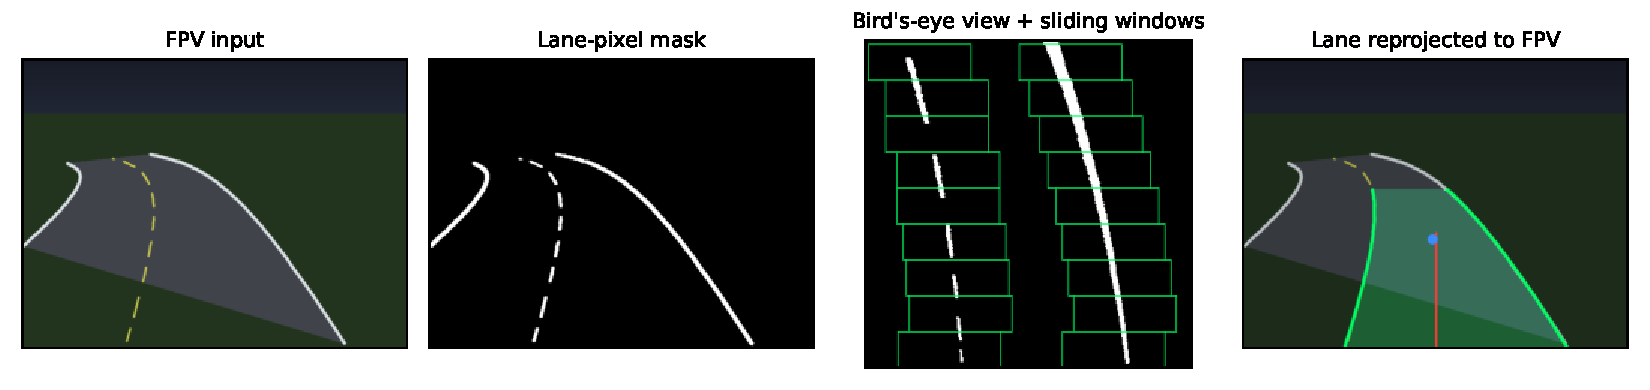
\includegraphics[width=\textwidth]{figures/polyfit_pipeline.pdf}
  \caption{Proposed polynomial-fit detector. From left to right:
    raw forward-perspective frame; combined Sobel-x + HSV lane-pixel
    mask; bird's-eye view with sliding windows superimposed; lane
    polygon reprojected to the camera frame, with the look-ahead point
    marked in blue.}\label{fig:pipeline}
\end{figure*}

\subsection{Controllers}
The default controller is a discrete PID
$\delta_t=K_p e_t + K_i\!\sum e_\tau\Delta t + K_d \dot{e}_t$ with
$K_p{=}1.2$, $K_i{=}0.008$, $K_d{=}0.5$ and integral anti-windup at
$\pm 50$. We additionally implement the Stanley law
$\delta=\psi+\arctan\!\big(k\,e_\perp/(k_s+v)\big)$ with $k{=}0.6$,
$k_s{=}20$, driven from the \emph{true} track geometry, as a
perception-free upper-bound reference. The gap between
PID-on-detection and Stanley-on-truth quantifies how much error the
perception pipeline alone introduces.

\section{Experiments}

\subsection{Setup}
All runs use the per-track design speeds (75--120\,px/s) and a
$\Delta t = 1/60$\,s simulation step. Each run is a single closed lap
from the spawn waypoint; a lap is \emph{completed} if the car returns
to within 40\,px of spawn without exceeding 0.5$\times$road-width
deviation for more than 1.5\,s. We report mean and RMS absolute
lateral error, max deviation, mean lane-IoU (predicted vs.\
ground-truth lane polygons), and mean detector inference time.

\subsection{Method comparison}
Table~\ref{tab:main} and Fig.~\ref{fig:rms} summarise the headline
result. The centroid baseline DNFs every track---it tracks the road
blob, not the lane centre, so any bend produces an accumulating bias.
Hough completes every track but oscillates near the lane centre
(25.4\,px mean RMS). The polynomial-fit detector reduces this to
16.6\,px ($\mathbf{-34\,\%}$) and lifts mean lane-IoU from 0.24 to
0.33 ($+38\,\%$). Stanley-on-truth achieves $<1$\,px RMS on every
track, establishing the order of magnitude of error the perception
alone is responsible for.

\begin{table}[h]
  \centering\scriptsize
  \begin{tabular}{l l r r r r r r}
\toprule
Track & Detector & Lap & RMS px & Mean px & Max px & IoU & ms/det \\
\midrule
Simple Oval & centroid & DNF & 99.5 & 80.0 & 194.3 & 0.01 & 1.15 \\
Simple Oval & hough & \checkmark & 27.4 & 27.2 & 28.7 & 0.17 & 0.75 \\
Simple Oval & polyfit & \checkmark & 17.6 & 16.9 & 27.2 & 0.25 & 1.92 \\
\midrule
Stadium Circuit & centroid & DNF & 39.5 & 32.8 & 113.4 & 0.39 & 1.79 \\
Stadium Circuit & hough & \checkmark & 26.2 & 26.0 & 30.1 & 0.24 & 0.77 \\
Stadium Circuit & polyfit & \checkmark & 17.0 & 16.3 & 23.6 & 0.31 & 1.94 \\
\midrule
Winding Road & centroid & DNF & 33.9 & 28.2 & 97.8 & 0.41 & 1.84 \\
Winding Road & hough & \checkmark & 24.9 & 24.7 & 28.4 & 0.23 & 0.76 \\
Winding Road & polyfit & \checkmark & 15.7 & 14.8 & 23.7 & 0.35 & 1.96 \\
\midrule
Grand Prix Circuit & centroid & DNF & 35.0 & 28.4 & 108.4 & 0.43 & 1.91 \\
Grand Prix Circuit & hough & \checkmark & 24.8 & 24.6 & 27.8 & 0.26 & 0.77 \\
Grand Prix Circuit & polyfit & \checkmark & 17.7 & 16.1 & 34.5 & 0.36 & 1.95 \\
\midrule
Highland Rally & centroid & DNF & 65.6 & 52.9 & 127.6 & 0.00 & 1.22 \\
Highland Rally & hough & \checkmark & 23.8 & 23.6 & 26.1 & 0.31 & 0.78 \\
Highland Rally & polyfit & \checkmark & 15.1 & 14.2 & 21.9 & 0.39 & 1.95 \\
\midrule
Red Bull Ring & centroid & DNF & 117.7 & 95.0 & 228.4 & 0.01 & 1.12 \\
Red Bull Ring & hough & \checkmark & 31.0 & 30.5 & 51.9 & 0.21 & 0.73 \\
Red Bull Ring & polyfit & DNF & 28.5 & 22.8 & 82.0 & 0.24 & 1.90 \\
\midrule
Simple Oval & Stanley (oracle) & \checkmark & 0.4 & 0.4 & 1.2 & 0.52 & 2.04 \\
\bottomrule
\end{tabular}
  \caption{Per-track RMS lateral error (camera px) and mean lane-IoU
    over one closed lap.\label{tab:main}}
\end{table}

\begin{figure}[h]
  \centering
  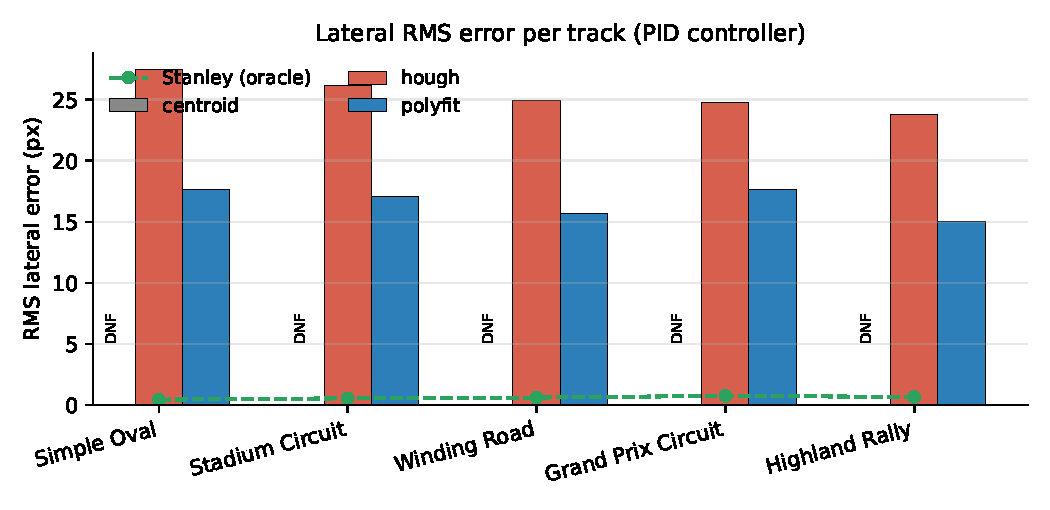
\includegraphics[width=\columnwidth]{figures/rms_by_track.pdf}
  \caption{RMS lateral error per track for the three detectors (PID).
    Stanley + truth is the dashed reference.}\label{fig:rms}
\end{figure}

\subsection{Per-frame behaviour on a curve}
Fig.~\ref{fig:annot} shows the three detectors on the same frame six
seconds into the Winding Road. The centroid sees a single blob and
reports a near-zero offset even though the lane curves right; Hough
fits a straight line that already underestimates the turn; the
polynomial detector traces the entire S-curve and produces a
look-ahead point that anticipates the upcoming bend. The corresponding
offset traces over the full lap (Fig.~\ref{fig:traces}) show the true
error of the polyfit run staying within $\pm 25$\,px while Hough
oscillates from $-40$ to $+30$\,px.

\begin{figure}[h]
  \centering
  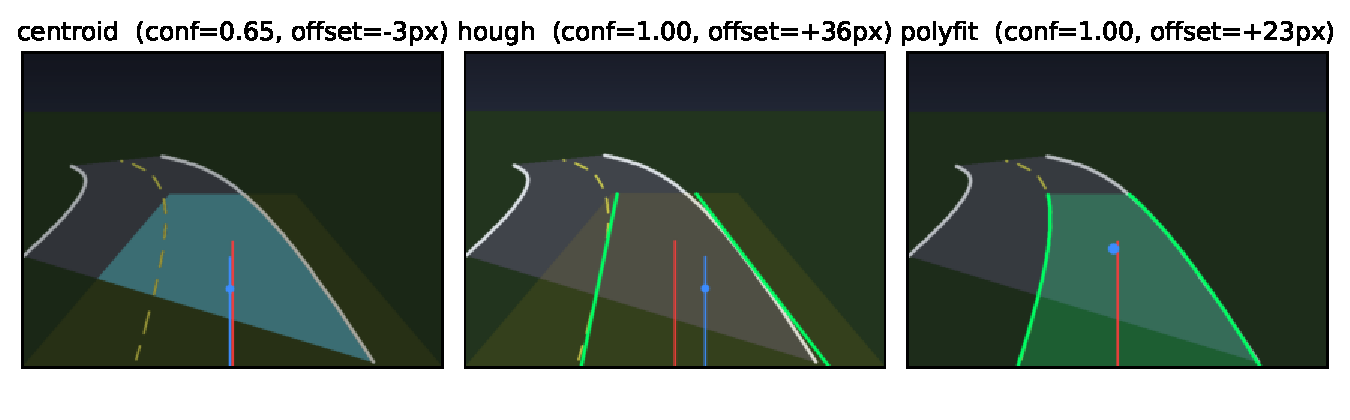
\includegraphics[width=\columnwidth]{figures/annotations.pdf}
  \caption{Same frame, three detectors. Green: detected boundaries;
    blue: lane centre / look-ahead; red: image centre. Hough fits a
    straight line through a curve; polyfit captures the bend.}\label{fig:annot}
\end{figure}

\begin{figure}[h]
  \centering
  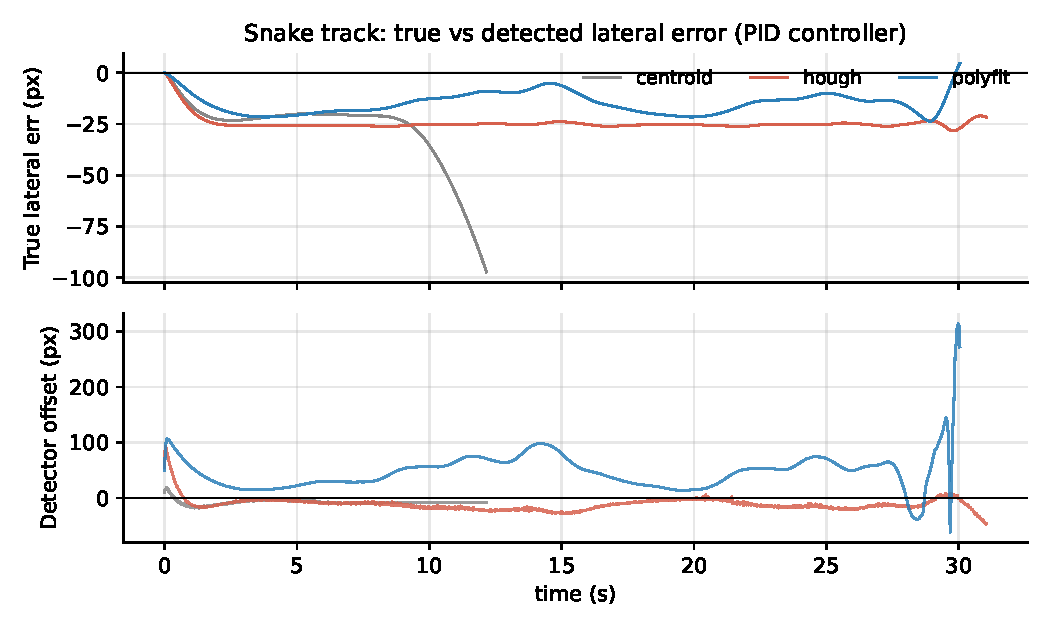
\includegraphics[width=\columnwidth]{figures/snake_traces.pdf}
  \caption{Per-frame lateral error on the Winding Road. Top:
    ground-truth error; bottom: detector-reported offset.
    Polyfit tracks the true error closely; Hough is biased on
    every bend.}\label{fig:traces}
\end{figure}

\subsection{Robustness to camera noise}
We re-ran the oval for each detector with i.i.d.\ Gaussian noise of
standard deviation $\sigma\in\{0,0.02,0.05,0.10,0.20\}$ added to every
frame (Fig.~\ref{fig:noise}). Centroid fails at every $\sigma$; Hough
is unaffected up to $\sigma=0.10$ but loses the lane at $\sigma=0.20$
because the noise overwhelms Canny's gradient. The polynomial-fit
detector completes the lap at every $\sigma$---its mask, which combines
a normalised Sobel-x response with two colour masks, is much less
sensitive to additive intensity noise.

\begin{figure}[h]
  \centering
  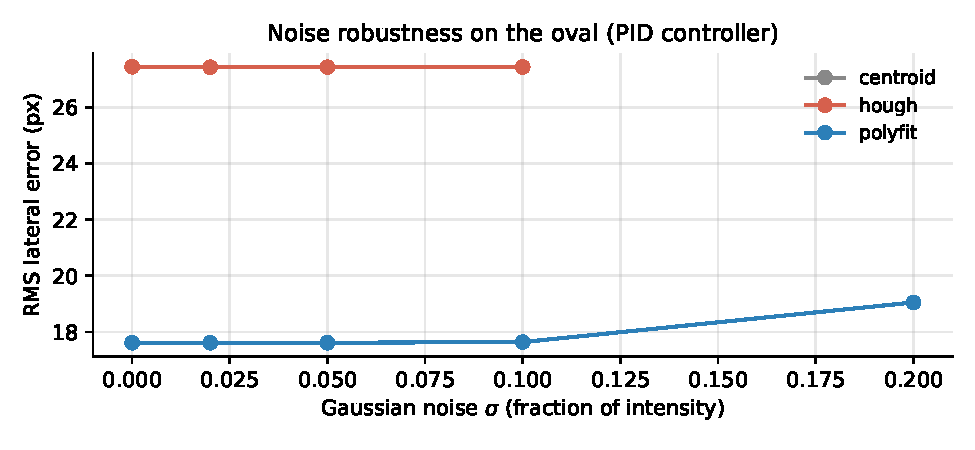
\includegraphics[width=\columnwidth]{figures/noise.pdf}
  \caption{Noise robustness on the oval (PID). Polyfit is the most
    stable.}\label{fig:noise}
\end{figure}

\subsection{Compute cost}
Mean detector inference time is 0.7\,ms (Hough) and 1.9\,ms (polyfit)
on a single CPU thread---$>1400$ and $>500$\,FPS respectively. The
polyfit overhead is dominated by the perspective warp and
\texttt{np.polyfit}, not by the sliding window.

\section{Discussion}

\textbf{What worked.} The look-ahead offset is the single biggest
contributor. With it disabled (using the bottom-of-image offset only)
the polyfit's RMS improvement shrinks from $\sim40\,\%$ to
$\sim10\,\%$. The polynomial fit is what makes the look-ahead reliable:
a straight-line model evaluated half-way up the image is a wild
extrapolation on a curve.

\textbf{Failure modes.} On extremely tight turns (Highland Rally
summit hairpins), all three detectors briefly lose one boundary as the
lane bends out of frame. The polyfit's temporal EMA recovers within a
few frames; the Hough detector lingers on its last good line and
introduces a transient bias. The centroid fails for a structural
reason: the moment of the road region is biased away from the
centreline whenever the road is asymmetric in the field of view.

\textbf{Where Stanley wins.} The Stanley + truth oracle gets to
sub-pixel RMS because it knows the path. Closing that gap requires
sub-pixel-accurate perception, which classical line detectors cannot
deliver without sub-pixel edge refinement. A learned segmenter would
be the next step.

\textbf{Limitations.} The simulator paints a perfectly consistent road
under controlled lighting, so our numbers are an upper bound on
real-world classical-CV performance. We also fix one speed schedule
per track; sweeping speed would likely favour the polyfit further (it
does not rely on the bottom of the image aligning with the car).

\section{Conclusion}
A modest upgrade---bird's-eye warp + sliding-window quadratic
fit---cuts the RMS lateral error of a classical lane-keeping pipeline
by more than a third on curved tracks while remaining real-time and
fully interpretable. Pairing the resulting look-ahead offset with a
plain PID closes most of the gap to a Stanley controller driven from
ground truth.

{\footnotesize\textbf{Reproducibility.} \texttt{python experiments.py}
followed by \texttt{python make\_qualitative\_figures.py} reproduces
every CSV and figure in this report (deterministic except for the noise
experiment, seeded by NumPy's default RNG). The simulator is launched
with \texttt{python main.py --detector polyfit --controller pid}.}

\end{document}
